\section{Thursday, April 23rd}
\subsection{Logistics}
\begin{itemize}
    \item Discussion due Thurs
    \item Consulting OH form
    \item Quiz 8 on Thurs (Scope: Last unit up until today, Source Channel Separation Thm.)
\end{itemize}

\subsection{Goals}
\begin{itemize}
    \item Achievability of Capacity
    \item AEP for ergodic sources
    \item Source-Channel Separation
\end{itemize}

\subsection{Channel Coding Theorem}
For a discrete, memoryless channel:
\begin{enumerate}
    \item Any rate $R<C$ is achievable
    \item If $R$ is achievable, then $R\leq C$. (We showed this last time)
\end{enumerate}
where:
$$
C = \max_{P_x} \left\{I[X; Y]\right\}
$$

\begin{proof}
\begin{itemize}
    \item 
All we need is to find a code that achieves $R, R\nearrow C$.
    \item 
Construct a \underline{random code}:
\end{itemize}
\begin{enumerate}
    \item Fix $p_x$
    \item Sample codewords $x^{(n)}(\omega) \{X_i(\omega)\}_{i=1}^n\simiid p_x$. Do this $d^{nR}$ for a base $d$, you have $d$ possible outcomes, to define the codebook.
    \item Sample codewords $x^{(n)}(\omega) \{X_i(\omega)\}_{i=1}^n\simiid p_x$. Do this $d^{nR}$ for a base $d$, you have $d$ possible outcomes, to define the codebook (code): $C$.
    \item Sender \& Receiver know $C, P_{Y|X}$.
    \item $W\sim \Uniform(\cW), \ |\cW|=d^{nR}$.
    \item Encode $W\to X^{(n)}(\omega)$.
    \item Send $X^{(n)}\stackrel{\to}{P_{Y|X}} Y^{(n)}$.
    \item Decode $Y^{(n)}{\to}\what\approx \omega$.
\end{enumerate}
\end{proof}

\subsection{Feedback Capacity Theorem}
The operational capacity w/ feedback is still $C =$ info capacity.

\subsection{Joint AEP Theorem}
$\left(X^{(n)}, Y^{(n)}\right)\sim P_{x^n, y^{(n)}}, \quad \left(X_j, Y_j\right)_{j=1}^n\simiid P_{x, y}$\\
then: 
\begin{enumerate}
    \item[(a)] $\Pr(\left(X^{(n)}, Y^{(n)}\right))$ is j.t. $\to1$ as $n\to\infty$. (almost all sequences $\sim P_{\left(X^{(n)}, Y^{(n)}\right)}$ are j.t.
    \item[(b)] If $\left(x^{(n)}, y^{(n)}\right)$ is j.t. then $\Pr(\left(X^{(n)}, Y^{(n)}\right)=\left(x^{(n)}, y^{(n)}\right))\in d^{-n(H[X, Y] \pm \varepsilon)}$
    \item[(c)] 
    \begin{align*}
    |\text{Jointly typical set}| 
        &\leq d^{n(H[X, Y] + \varepsilon)}
        \\
        &\geq (1-\varepsilon) d^{n(H[X, Y]-\varepsilon)}
        &&\text{ for $n$ large enough}
    \end{align*}
The set of j.t. sequences is (relatively) small.
\item[(d)] If $\tilde{X}^{(n)}\sim p_{x^n}, \tilde{Y}^{(n)}\sim p_{y^n}, \tilde{X}\indep \tilde{Y}$ then: 
\begin{align*}
\Pr(\left(\tilde{X}^{(n)}, \tilde{Y}^{(n)}\right)\text{ is j.t.})
    &\leq d^{-n(I[X; Y] - 3\varepsilon)}
    \\
    &\geq (1-\varepsilon) d^{-n(I[X; Y] + 3\varepsilon)}
        &&\text{ for $n$ large enough}
\end{align*}
$\indep$ly typical sequences are \underline{rarely} j.t.
\end{enumerate}

\begin{figure}[h]
    \centering
    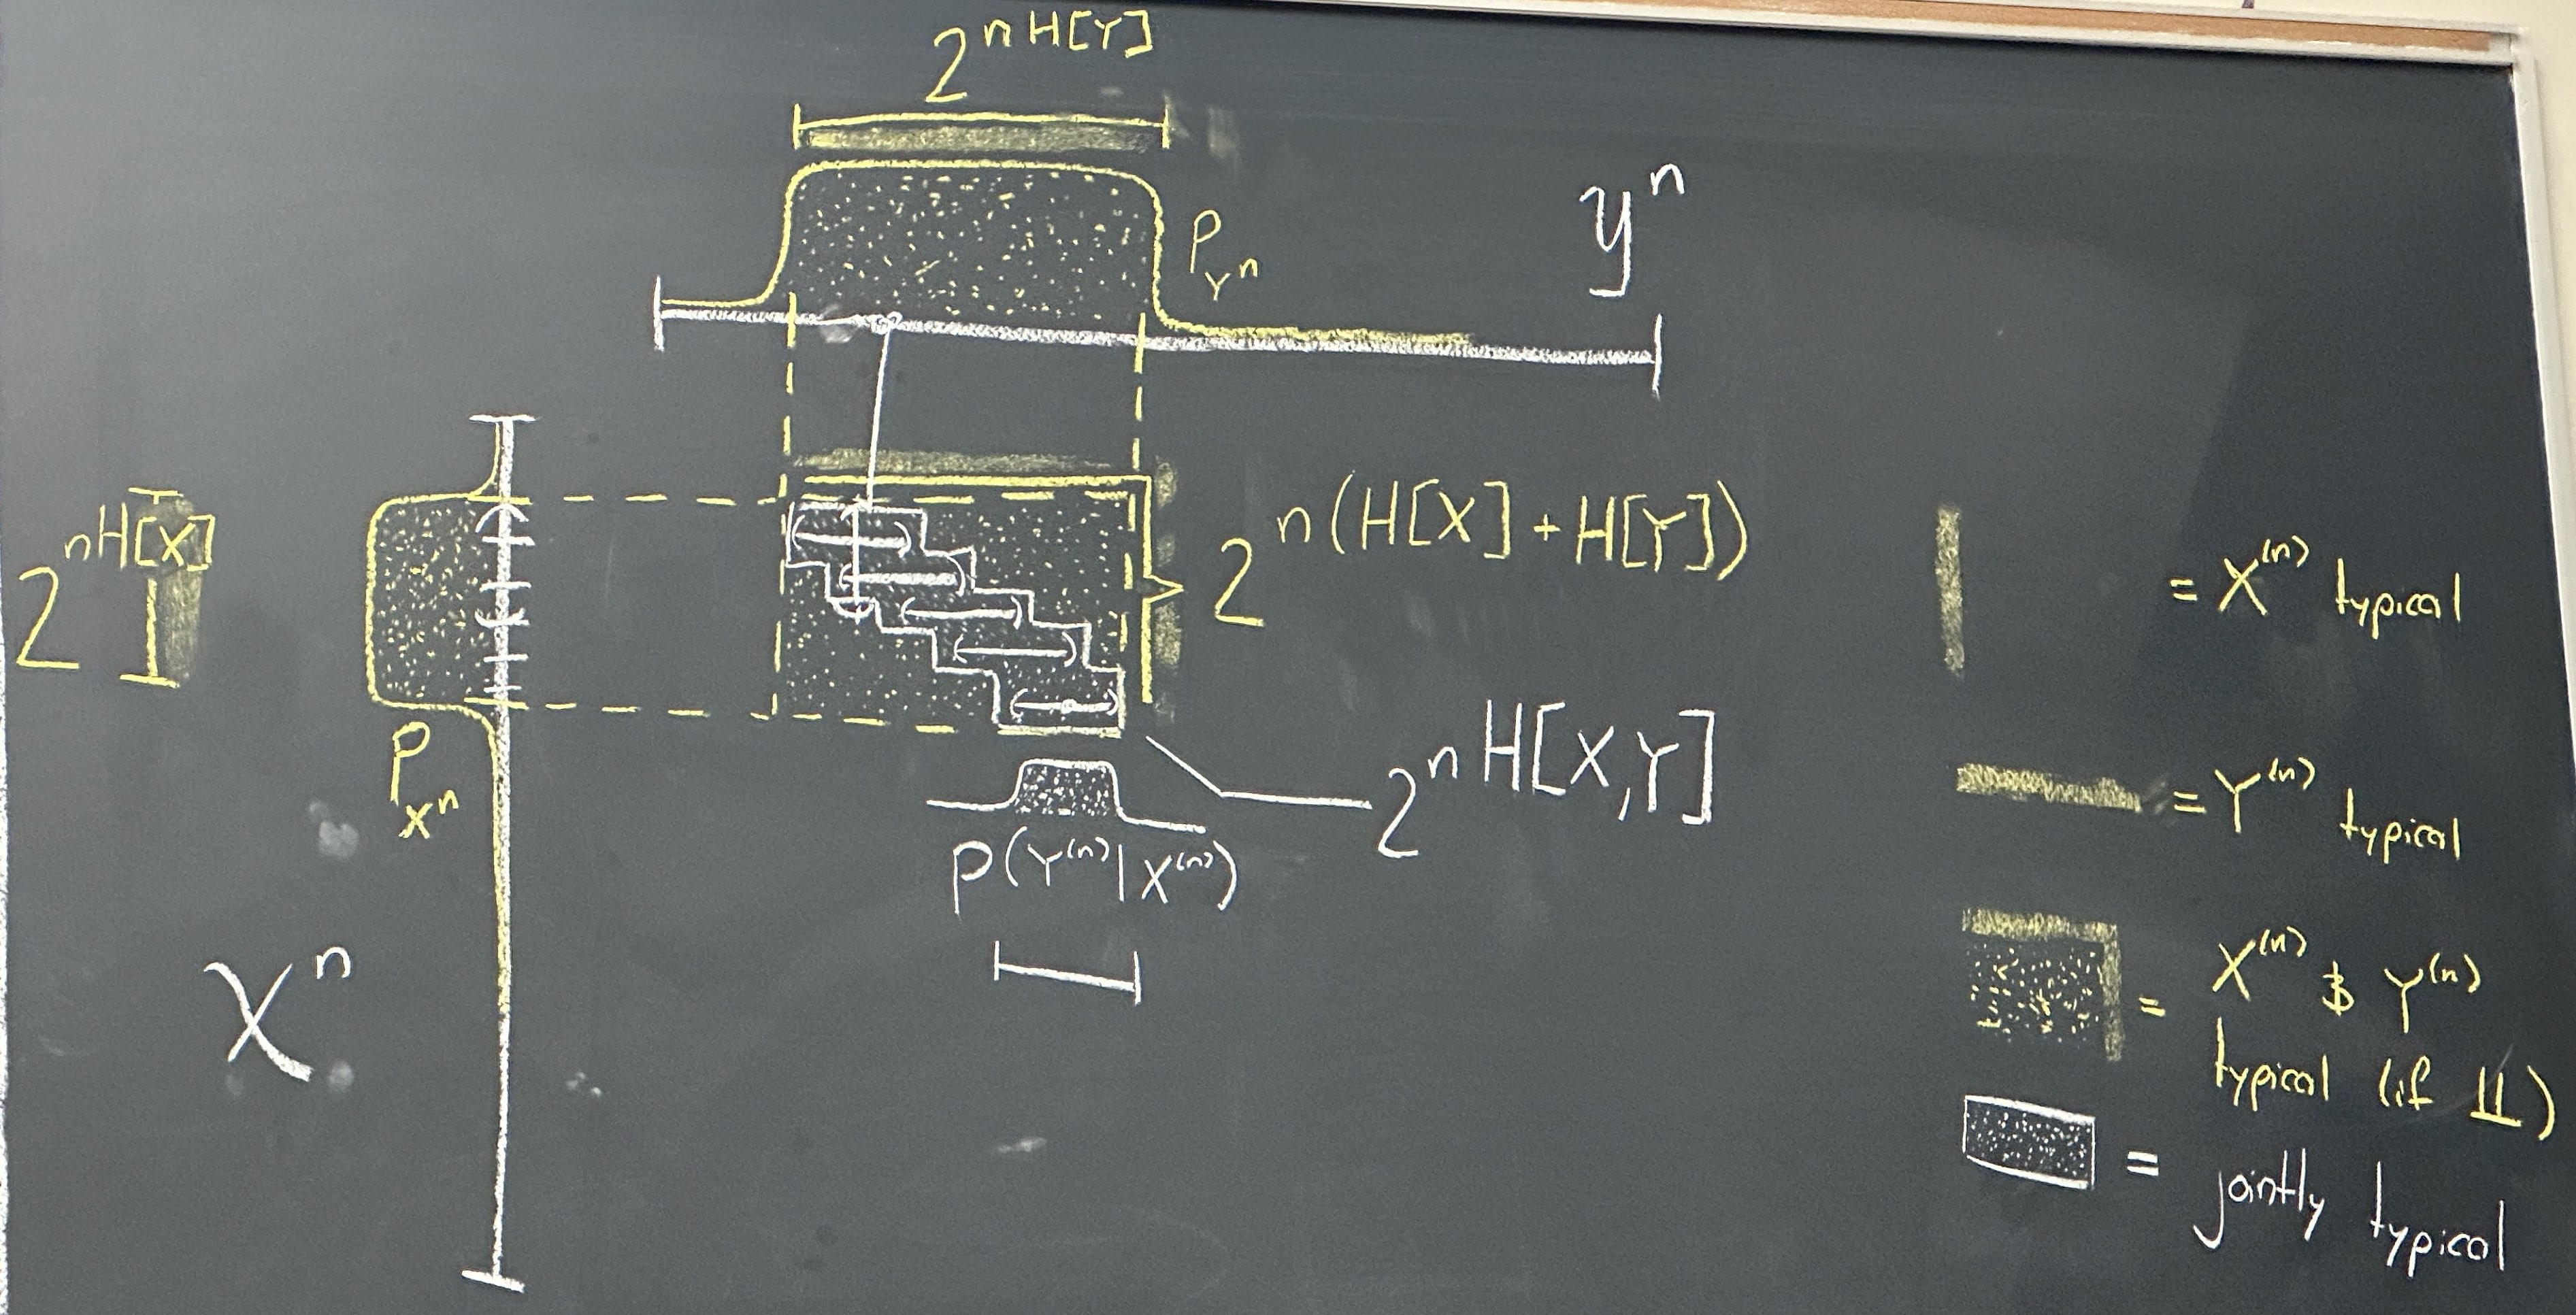
\includegraphics[scale=0.14]{lectures/wk13/img/strip.jpg}
    % \caption{Diagonal Strip}
    \label{fig:strip}
\end{figure}

Here we can see that $\cX^n$ is the input and $y^n$ is the output, we know that we can adjust $\varepsilon$

\subsubsection{How to decode?}
Using j.t., we let $JT(\omega') = \{\left(\tilde{X}^{(n)}(\omega'), \tilde{Y}^{(n)}\right) \text{ is j.t.}\}$.

We decode by looking for an input message $\omega'$ which is j.t. with the received signal $Y^{(n)}$. If there are multiple (we cannot decode properly then we return an error).

\subsubsection{When do we error?}
We error in 2 cases:
\begin{enumerate}
    \item If $JT(\omega)^c=X^{(n)}(\omega)$ is not j.t. w/ $Y^{(n)}$.
    \item If $\exists\omega'\neq\omega\st JT(\omega'), X^{(n)}(\omega')$ is also j.t. with $Y^{(n)}$.
\end{enumerate}

\subsubsection{Detailed Error Analysis}
\begin{flalign*}
\Pr(\text{error}) 
    &= \E_C[\Pr(\text{error} \mid C)] \\
    &= \E_C[\E_W[\Pr(\text{error} \mid C, W)]] \\
    &= \E_{C, W}[\Pr(\text{error} \mid C, W)] \\
    &= \E_{C}[\Pr(\text{error} \mid C, W=1)] \\
    &= \Pr(\text{error} \mid W=1) \\
    &= \Pr(JT(1)^c \cup (\bigcup_{\omega \neq1} JT(\omega)) \mid W=1) \\
    &\leq \underbrace{\Pr(JT(1)^c \mid W=1)}_{\underbrace{Y^{(n)}\text{ is not j.t. w/ } X^{(n)}(1)}_{\leq\varepsilon}}
    + \sum_{\omega \neq1}\Pr(JT(\omega') \mid W=1) 
    &&[\text{Apply Union Bound}] \\
    \Pr(JT(1)^c \mid W=1)
        &\leq \varepsilon \text{ for large } n
    &&[\text{by AEP}] \\
    % \implies \Pr(\text{error}) &\leq \varepsilon + \sum_{\omega \neq1}\Pr(\underbrace{JT(\omega') \mid W=1}_{\underbrace{\stackrel{W=1\to X^{(n)}(1)\to Y^{(n)}}{\omega'\neq 1\to X^{(n)}(\omega')}}_{\left(\tilde{X}^{(n)}(\omega'), \tilde{Y}^{(n)}\right)\text{ drawn }\indep\text{ly of }X^{(n)}(1), X^{(n)}(\omega')\indep Y^{(n)} \text{ if }\omega'\neq1}) \\
        &\leq \varepsilon +\sum_{\omega'\neq1} d^{-n(I[X; Y] -3\varepsilon)} \\
        &\leq \varepsilon +\sum_{\omega'\neq1} d^{nR} d^{-n(I[X; Y] -3\varepsilon)} \\
        &\leq \varepsilon +\sum_{\omega'\neq1} d^{-n((I[X; Y] -3\varepsilon) - R)}
\end{flalign*}
If $R < I[X; Y]-3\varepsilon$ then $d^{-n(\ldots)}\searrow0$ as $n\to\infty$. If $R < I[X; Y]-3\varepsilon, \exists n$ large enough $\st\Pr(\text{error})\leq 2\varepsilon$.

\subsection{Source Model}
Suppose $\cW$ is a stochastic process. 
\begin{align*}
    W^{(n)}=\{W_i\}_{i=1}^n\sim\cW
\end{align*}
This is producing new entropy every time I draw sample, which makes us take more to encode the information.

First extend the AEP to apply to stochastic sources: Recall that the AEP is, in essence, LLN. This means we can consider \underline{ergodic} (stationary) sources, where ergodic means that if we take a sample average over trajectories, it will be close to the population average.
\begin{align*}
    \lim_{T\to\infty}\frac{1}{T}\sum_{t=1}^{T} f(W_t) \ip \E_{W\sim P_s}[f(W)]
\end{align*}

\subsection{AEP: Shannon–McMillan–Breiman Theorem}
If $H$ is the entropy rate of a finite-valued stationary ergodic process $\left\{X_n\right\}$, then
$$
-\frac{1}{n} \log p\left(X_0, \ldots, X_{n-1}\right) \rightarrow H \quad \text { with probability } 1 .
$$

\subsection{Source-Separation Theorem}
Extension to the Channel Coding Theorem for Source: if given a stochastic source which satisfies the AEP, then we can transmit messages with vanishingly probability of error.

If $V_1, V_2, \ldots V^n$ is a finite alphabet stochastic process that satisfies the AEP and $H(\mathcal{V})<$ $C$, there exists a source-channel code with probability of error $\operatorname{Pr}\left(\hat{V}^n \neq\right.$ $\left.V^n\right) \rightarrow 0$. Conversely, for any stationary stochastic process, if $H(\mathcal{V})>C$, the probability of error is bounded away from zero, and it is not possible to send the process over the channel with arbitrarily low probability of error.

\subsection{What we have shown}
If $R<I[X ; y]-3 \varepsilon$, then for large $n$, average $P(\text{error})\leq 2\varepsilon$.

1. Use $P_x=P_x^*=\underset{P_x}{\operatorname{argmax}}\{I[X ; Y]\}$ then $I[X ; Y]=C$ then if $R<C$, average prob of error $\rightarrow 0$ as $n\to\infty$.

2. $\Pr(\text{error})=\mathbb{E}_{C}\left[P(\text{error} \mid C)\right] \leq 2 \varepsilon$ then $\exists C^\ast\st\Pr(\text{error}\mid C^\ast)\leq 2\varepsilon$.

3. \begin{align*}
\operatorname{Pr}\left(\text{error} \mid C^\ast\right) &\leq 2 \varepsilon.
\\
\operatorname{Pr}\left(\text{error} \mid C^\ast\right)
    &=\mathbb{E}_{W \sim \text{ Uniformly}(\cW)}\left[\operatorname{Pr}\left(\text{error} \mid C^\ast, W\right)\right] \leq 2 \varepsilon.
\end{align*}
There exists a set of messages $W\st\Pr(\text{error}\mid C^\ast, W)\leq 4\varepsilon$ and there are at least $|\cW|/2=\frac{2^{nR}}{2}=2^{nR-1}=2^{n(R-1/n)}$ and discard all other messages.

Provided $\displaystyle\lim _{n \rightarrow \infty} R^{\prime}=\lim _{n \rightarrow \infty}(R - 1 / n)<C$.


